\PassOptionsToPackage{unicode=true}{hyperref} % options for packages loaded elsewhere
\PassOptionsToPackage{hyphens}{url}
\documentclass[11pt,dvipsnames,ignorenonframetext,aspectratio=169]{beamer}
\IfFileExists{pgfpages.sty}{\usepackage{pgfpages}}{}
\setbeamertemplate{caption}[numbered]
\setbeamertemplate{caption label separator}{: }
\setbeamercolor{caption name}{fg=normal text.fg}
\beamertemplatenavigationsymbolsempty
\usepackage{lmodern}
\usepackage{amssymb,amsmath}
\usepackage{ifxetex,ifluatex}
\usepackage{fixltx2e} % provides \textsubscript
\ifnum 0\ifxetex 1\fi\ifluatex 1\fi=0 % if pdftex
  \usepackage[T1]{fontenc}
  \usepackage[utf8]{inputenc}
\else % if luatex or xelatex
  \ifxetex
    \usepackage{mathspec}
  \else
    \usepackage{fontspec}
\fi
\defaultfontfeatures{Ligatures=TeX,Scale=MatchLowercase}







\fi

  \usetheme[]{monash}

  \usecolortheme{monashwhite}


% A default size of 24 is set in beamerthememonash.sty
  \setbeamerfont{title}{series=\bfseries,parent=structure,size=\fontsize{18pt}{32}}

% Title page
\setbeamertemplate{title page}
{\placefig{-0.01}{-0.01}{width=1.01\paperwidth,height=1.01\paperheight}{fusrekhola\_falls\_kaski\_20210814.jpg}
\begin{textblock}{7.5}(1,2.8)\usebeamerfont{title}
{\color{white}\raggedright\par\inserttitle}
\end{textblock}
\begin{textblock}{7.5}(1,7)
{\color{white}\raggedright{\insertauthor}\mbox{}\\[0.2cm]
\insertdate}
\end{textblock}}


  \useinnertheme{rounded}

  \useoutertheme{smoothtree}

% use upquote if available, for straight quotes in verbatim environments
\IfFileExists{upquote.sty}{\usepackage{upquote}}{}
% use microtype if available
\IfFileExists{microtype.sty}{%
  \usepackage{microtype}
  \UseMicrotypeSet[protrusion]{basicmath} % disable protrusion for tt fonts
}{}


\newif\ifbibliography
  \usepackage[round]{natbib}
  \bibliographystyle{plainnat}


\hypersetup{
      pdftitle={Defence mechanisms against pathogens, parasites, insects},
            colorlinks=true,
    linkcolor=red,
    citecolor=Blue,
    urlcolor=lightgrayd,
    breaklinks=true}
%\urlstyle{same}  % Use monospace font for urls







% Prevent slide breaks in the middle of a paragraph:
\widowpenalties 1 10000
\raggedbottom

  \AtBeginPart{
    \let\insertpartnumber\relax
    \let\partname\relax
    \frame{\partpage}
  }
  \AtBeginSection{
    \ifbibliography
    \else
      \let\insertsectionnumber\relax
      \let\sectionname\relax
      \frame{\sectionpage}
    \fi
  }
  \AtBeginSubsection{
    \let\insertsubsectionnumber\relax
    \let\subsectionname\relax
    \frame{\subsectionpage}
  }



\setlength{\parindent}{0pt}
\setlength{\parskip}{6pt plus 2pt minus 1pt}
\setlength{\emergencystretch}{3em}  % prevent overfull lines
\providecommand{\tightlist}{%
  \setlength{\itemsep}{0pt}\setlength{\parskip}{0pt}}

  \setcounter{secnumdepth}{0}


%% Monash overrides
\AtBeginSection[]{
   \frame<beamer>{
   \frametitle{Outline}\vspace*{0.2cm}
   
   \tableofcontents[currentsection,hideallsubsections]
  }}

% Redefine shaded environment if it exists (to ensure text is black)
\ifcsname Shaded\endcsname
  \definecolor{shadecolor}{RGB}{225,225,225}
  \renewenvironment{Shaded}{\color{black}\begin{snugshade}\color{black}}{\end{snugshade}}
\fi
%%


  \usepackage{setspace}
  \usepackage{wasysym}
  % \usepackage{footnote} % don't use this this breaks all
  \usepackage{fontenc}
  \usepackage{fontawesome}
  \usepackage{booktabs,siunitx}
  \usepackage{longtable}
  \usepackage{array}
  \usepackage{multirow}
  \usepackage{wrapfig}
  \usepackage{float}
  \usepackage{colortbl}
  \usepackage{pdflscape}
  \usepackage{tabu}
  \usepackage{threeparttable}
  \usepackage{threeparttablex}
  \usepackage[normalem]{ulem}
  \usepackage{makecell}
  \usepackage{xcolor}
  \usepackage{tikz} % required for image opacity change
  \usepackage[absolute,overlay]{textpos} % for text formatting
  \usepackage{chemfig}
  \usepackage[skip=0.333\baselineskip]{caption}
  % \newcommand*{\AlignChar}[1]{\makebox[1ex][c]{\ensuremath{\scriptstyle#1}}}%
  \usepackage{siunitx}

  % this font option is amenable for beamer
  \setbeamerfont{caption}{size=\tiny}
  \singlespacing
  \definecolor{lightgrayd}{gray}{0.95}
  \definecolor{skyblued}{rgb}{0.65, 0.6, 0.94}
  \definecolor{oranged}{RGB}{245, 145, 200}

  % % better to insert it into template itself
  % \newlength{\cslhangindent}
  % \setlength{\cslhangindent}{1.5em}
  % \newenvironment{cslreferences}%
  %   {\setlength{\parindent}{0pt}%
  %   \everypar{\setlength{\hangindent}{\cslhangindent}}\ignorespaces}%
  %   {\par}

  \usepackage[caption=false]{subfig}

  \newcommand{\bcolumns}{\begin{columns}[T, onlytextwidth]}
  \newcommand{\ecolumns}{\end{columns}}

  \newcommand{\bdescription}{\begin{description}}
  \newcommand{\edescription}{\end{description}}

  \newcommand{\bitemize}{\begin{itemize}}
  \newcommand{\eitemize}{\end{itemize}}
  \AtBeginSubsection{}
  \newcommand{\bsmall}{\begin{small}}
  \newcommand{\esmall}{\end{small}}

  \title[]{Defence mechanisms against pathogens, parasites, insects}


  \author[
        \vspace{-0.5cm}Deependra Dhakal\\
Assistant Professor\\
Agriculture and Forestry University\\
\textit{ddhakal.rookie@gmail.com}\\
\url{https://rookie.rbind.io}
    ]{\vspace{-0.5cm}Deependra Dhakal\\
Assistant Professor\\
Agriculture and Forestry University\\
\textit{ddhakal.rookie@gmail.com}\\
\url{https://rookie.rbind.io}}


\date[
      
  ]{
    }

\begin{document}

% Hide progress bar and footline on titlepage
  \begin{frame}[plain]
  \titlepage
  \end{frame}


   \frame<beamer>{
   \frametitle{Outline}\vspace*{0.2cm}
   
   \tableofcontents[hideallsubsections]
  }

\hypertarget{mechanisms-of-infection}{%
\section{Mechanisms of infection}\label{mechanisms-of-infection}}

\begin{frame}{}
\protect\hypertarget{section}{}
\footnotesize

\begin{itemize}
\tightlist
\item
  Pathogens act in a variety of pathways to cause infection
\item
  In pathogens that show a high level of gene flow, greater genetic
  diversity exists
\item
  In pathogens reproducing asexually (with no recombination), entire
  genotypes are transferred from one population to another -- phenomena
  called genotype flow
\item
  Hardy spores or propagules (rust and powdery mildew) can spread over
  long distances, sometimes encompassing entire continents.
\item
  Soil-borne fungi and nematodes move slowly and are present in small
  areas.
\item
  Gene flow reduces genetic differences between populations, preventing
  delays in drastic evolution of the population in different
  geographical areas.
\item
  Population size affects phenomena such as mutation, genetic drift and
  selection

  \begin{itemize}
  \footnotesize
  \item $\Uparrow$ population size $\thicksim$ $\Uparrow$ mutants alleles are conserved
  \item $\Uparrow$ population size $\thicksim$ $\Uparrow$ rare alleles are preserved under genetic drift 
  \end{itemize}
\end{itemize}
\end{frame}

\begin{frame}{}
\protect\hypertarget{section-1}{}
\begin{figure}
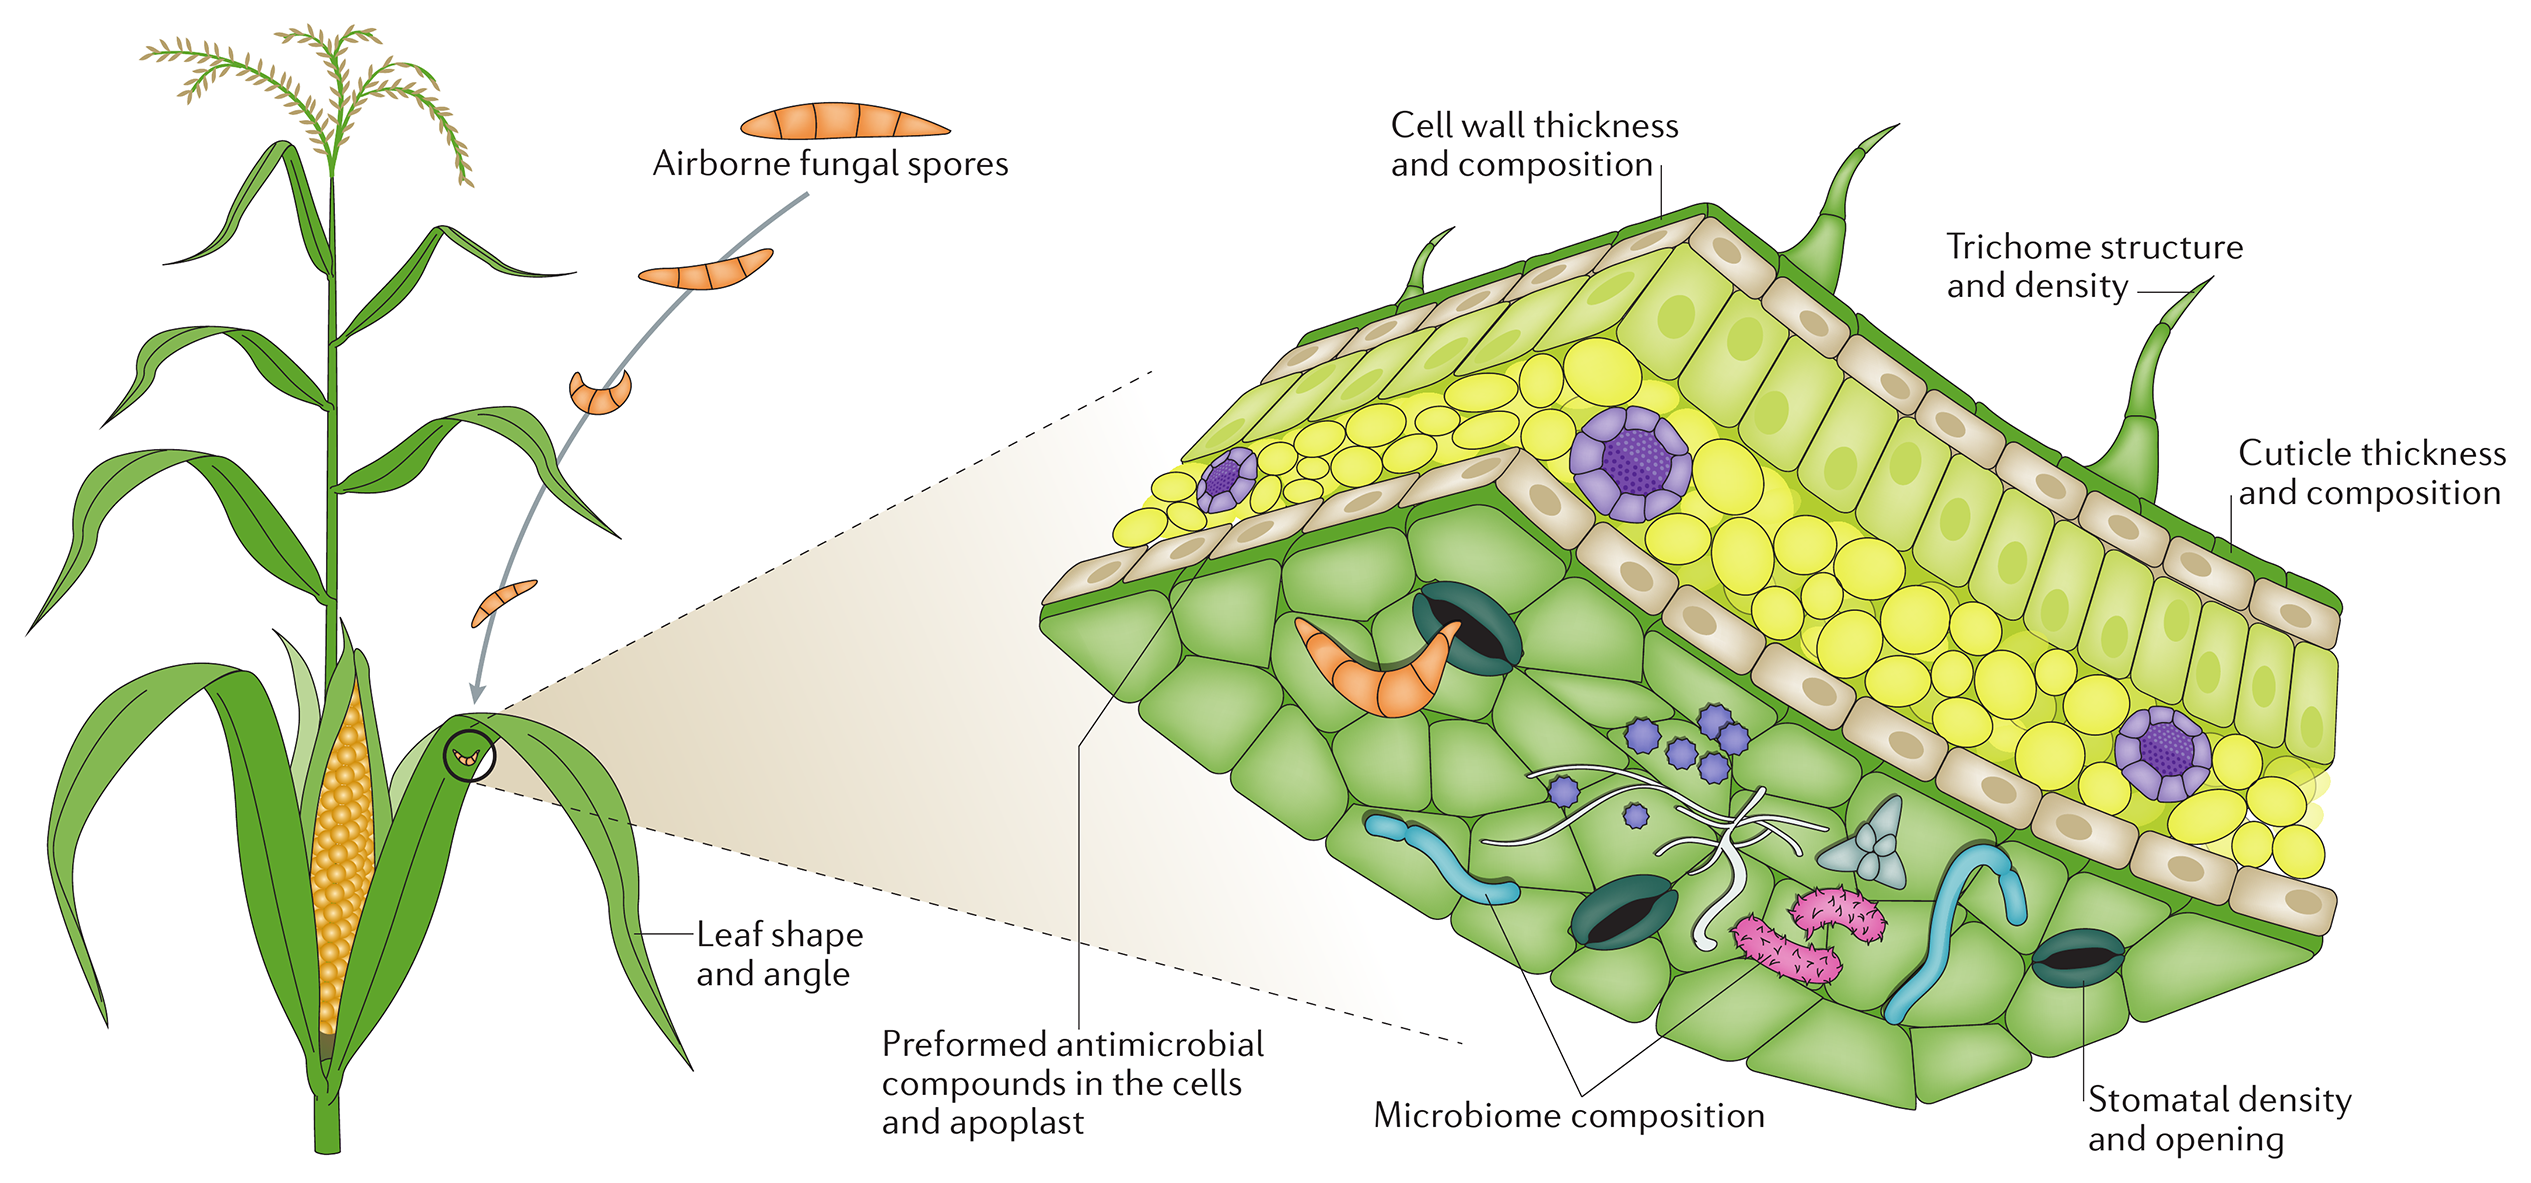
\includegraphics[width=0.8\linewidth]{../images/infection_process_plants_extracellular} \caption{Resistance mechanisms at the tissue level. At the organismal and tissue levels, the success of a pathogen can be influenced by a range of features of the morphology, biochemistry and microbiome of the plant.}\label{fig:infection-mechanism-extracellular}
\end{figure}
\end{frame}

\begin{frame}{}
\protect\hypertarget{section-2}{}
\begin{figure}
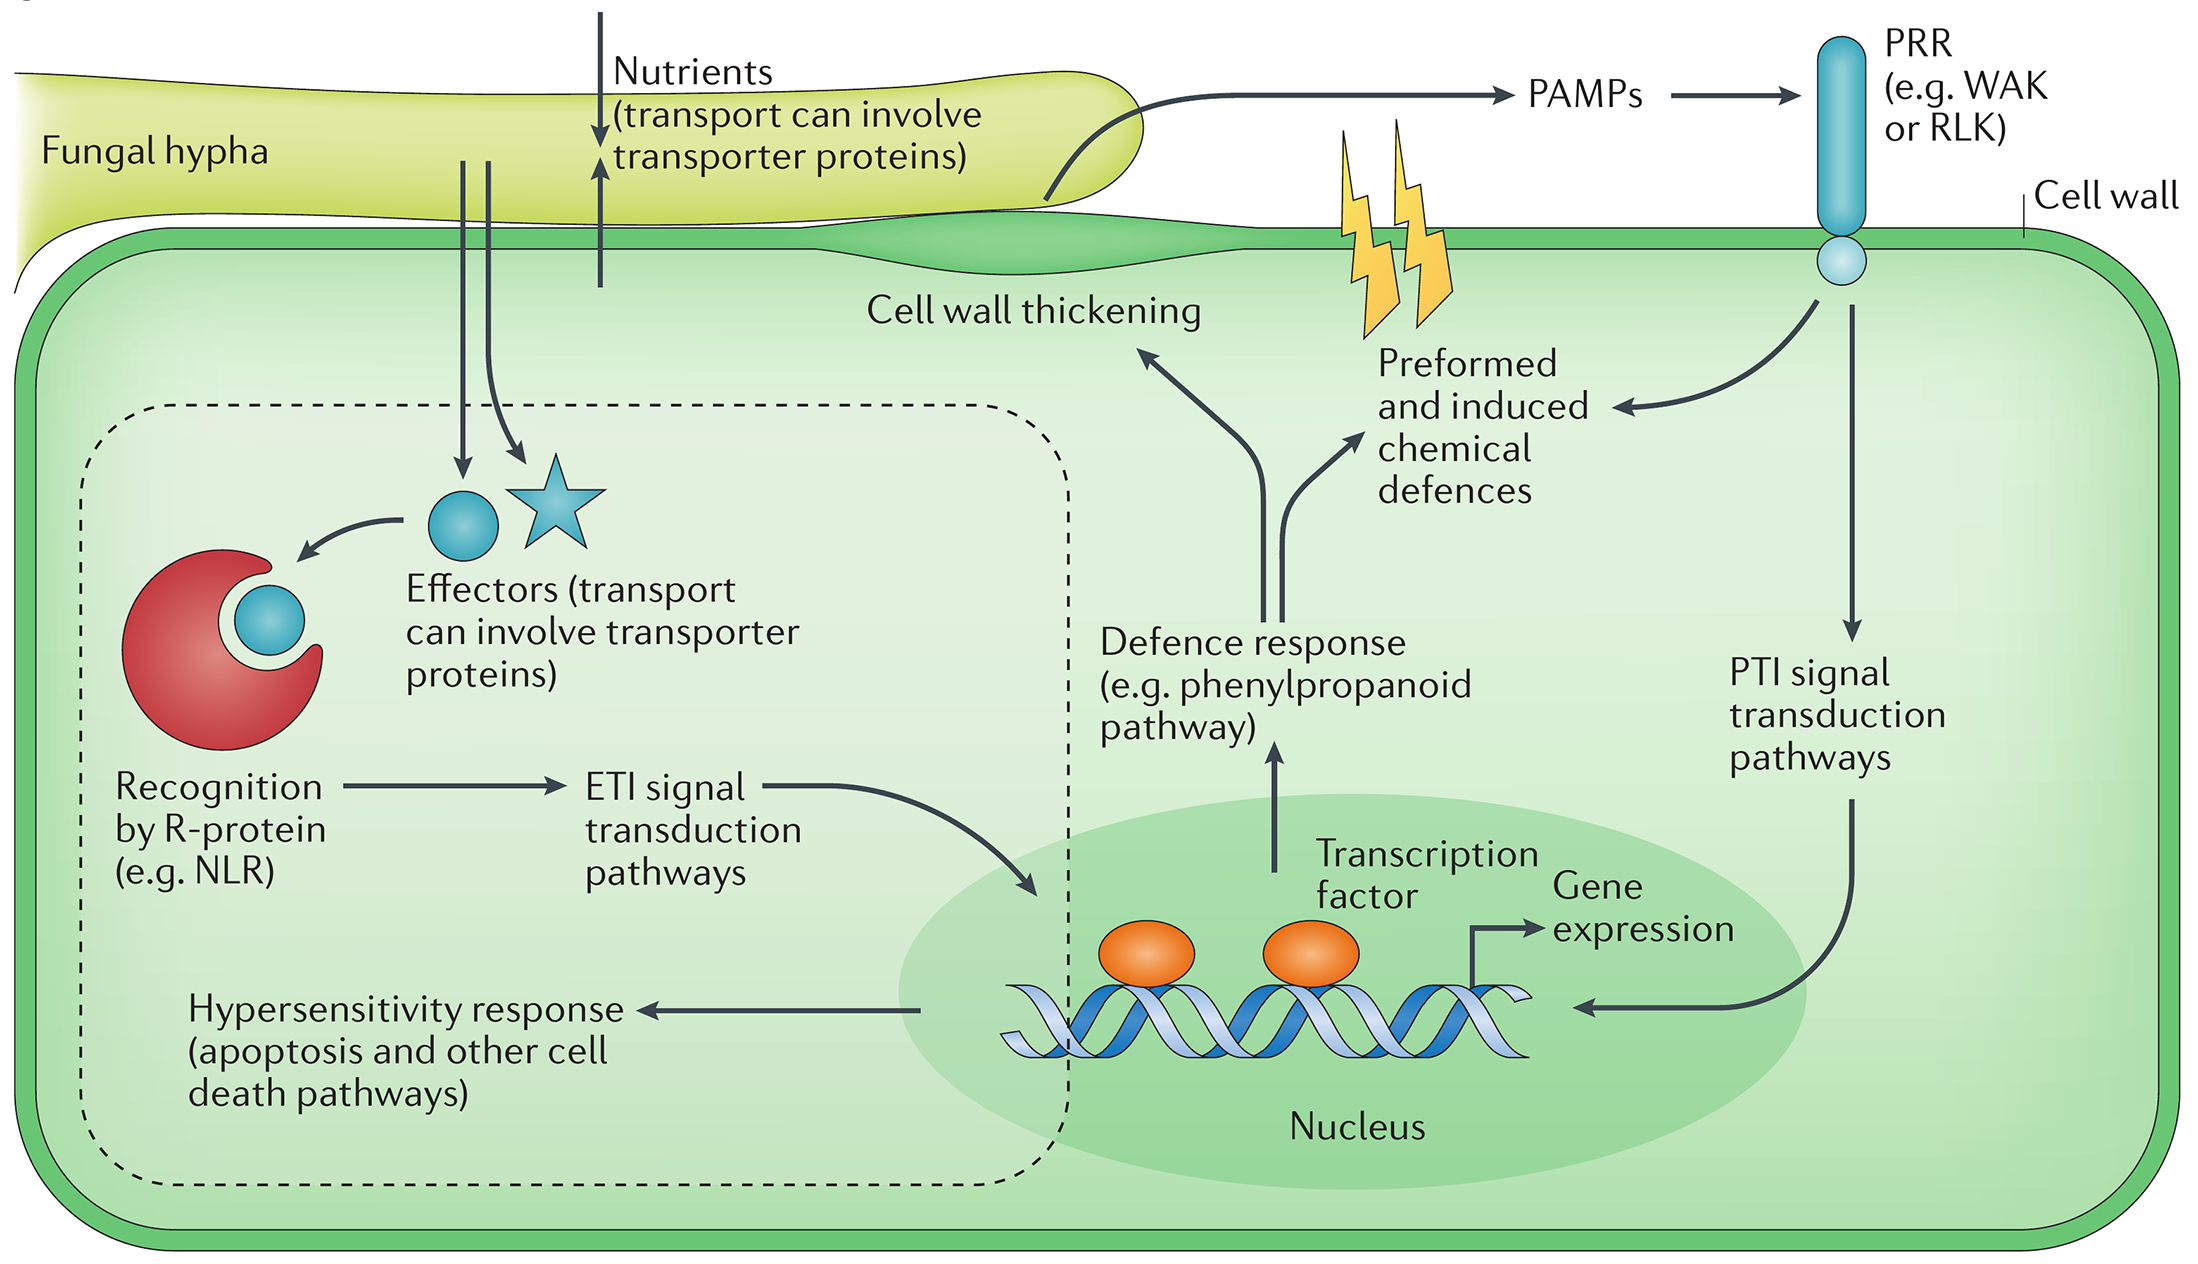
\includegraphics[width=0.78\linewidth]{../images/infection_process_plants_intracellular} \caption{At cellular level, factors that affect the ability of a pathogen to infect its plant host include defence responses triggered by recognition events in the host via PRRs, such as WAKs or RLKs, and resistance proteins (R-proteins), such as NLR proteins, nutrient availability in the apoplast and cytoplasm; pre-existing chemical factors; and cell wall constitution. These factors are affected by host genotype and are potential causes of quantitative variation. Qualitative variation in resistance usually, though not always, occurs at the level of resistance gene-effector interactions.}\label{fig:infection-mechanism-intracellular}
\end{figure}
\end{frame}

\begin{frame}{Physiology of defense}
\protect\hypertarget{physiology-of-defense}{}
\begin{itemize}
\tightlist
\item
  In many cases of host-pathogen interaction, genes in one organism are
  triggered to be expressed by a substance produced by the other
  organism. For example,

  \begin{itemize}
  \tightlist
  \item
    genes for cell wall-degrading enzymes in the pathogen are induced by
    the presence of monomers or oligomers of host cell wall
    macromolecules that are substrates for these enzymes.
  \item
    genes for defense reactions in the host, eg. phytoalexins, are
    triggered to expression by certain signal compounds activated by
    inducer molecules (elicitors) produced by the pathogen.
  \end{itemize}
\end{itemize}
\end{frame}

\hypertarget{genetics-of-disease-and-resistance-mechanism}{%
\section{Genetics of disease and resistance
mechanism}\label{genetics-of-disease-and-resistance-mechanism}}

\begin{frame}{}
\protect\hypertarget{section-3}{}
\bcolumns
\column{0.5\textwidth}
\small

\begin{itemize}
\tightlist
\item
  In order to understand disease, genetics of causal agent need to be
  elucidated
\item
  Characters in individuals including pathogens are variable mostly as a
  result of

  \begin{itemize}
  \footnotesize
  \item Sexual process -- oospores, ascospores and basidiospores (in oomycetes and fungi); seeds of higher plants and eggs of nematodes
  \item Asexual process -- (owing to astronomical number of microorganism individuals produced) conidia, zoospores, sclerotia and uredospores (in fungi); bacteria, mollicutes and viruses
  \end{itemize}
\item
  Sexually reproducing organisms generate variability through
  segregation and recombination of genes, and even in asexually
  reproducing pathogens (bacteria) variants are produced by mutations.
\end{itemize}

\column{0.5\textwidth}

\footnotesize

\begin{itemize}
\tightlist
\item
  Genetic information (determines the form and function) is encoded as
  DNA or (exceptionally) RNA.

  \begin{itemize}
  \scriptsize
  \item Nucleus (follows Mendalian inheritance)
  \item Mitochondria
  \item Plasmid (autonomously replicating)
  \item Chloroplasts
  \end{itemize}
\item
  A gene (in general) is characterized by:

  \begin{itemize}
  \scriptsize
  \item 100-500 codon triplets
  \item Coding and and non-coding region
  \item Protein or RNA as code product
  \end{itemize}
\item
  Genetic processes

  \begin{itemize}
  \scriptsize
  \item Replication
  \item Transcription
  \item Translation
  \item Regulatory elements -- promoters, enhancers, silencers or terminators
  \end{itemize}
\end{itemize}

\ecolumns
\end{frame}

\begin{frame}{}
\protect\hypertarget{section-4}{}
\begin{itemize}
\tightlist
\item
  Factors affecting gene flow and genotype fitness are major drivers for
  evolution of both plant pathogen and host population
\item
\end{itemize}
\end{frame}

\begin{frame}{Genetic processes involved in infection}
\protect\hypertarget{genetic-processes-involved-in-infection}{}
\begin{figure}

{\centering 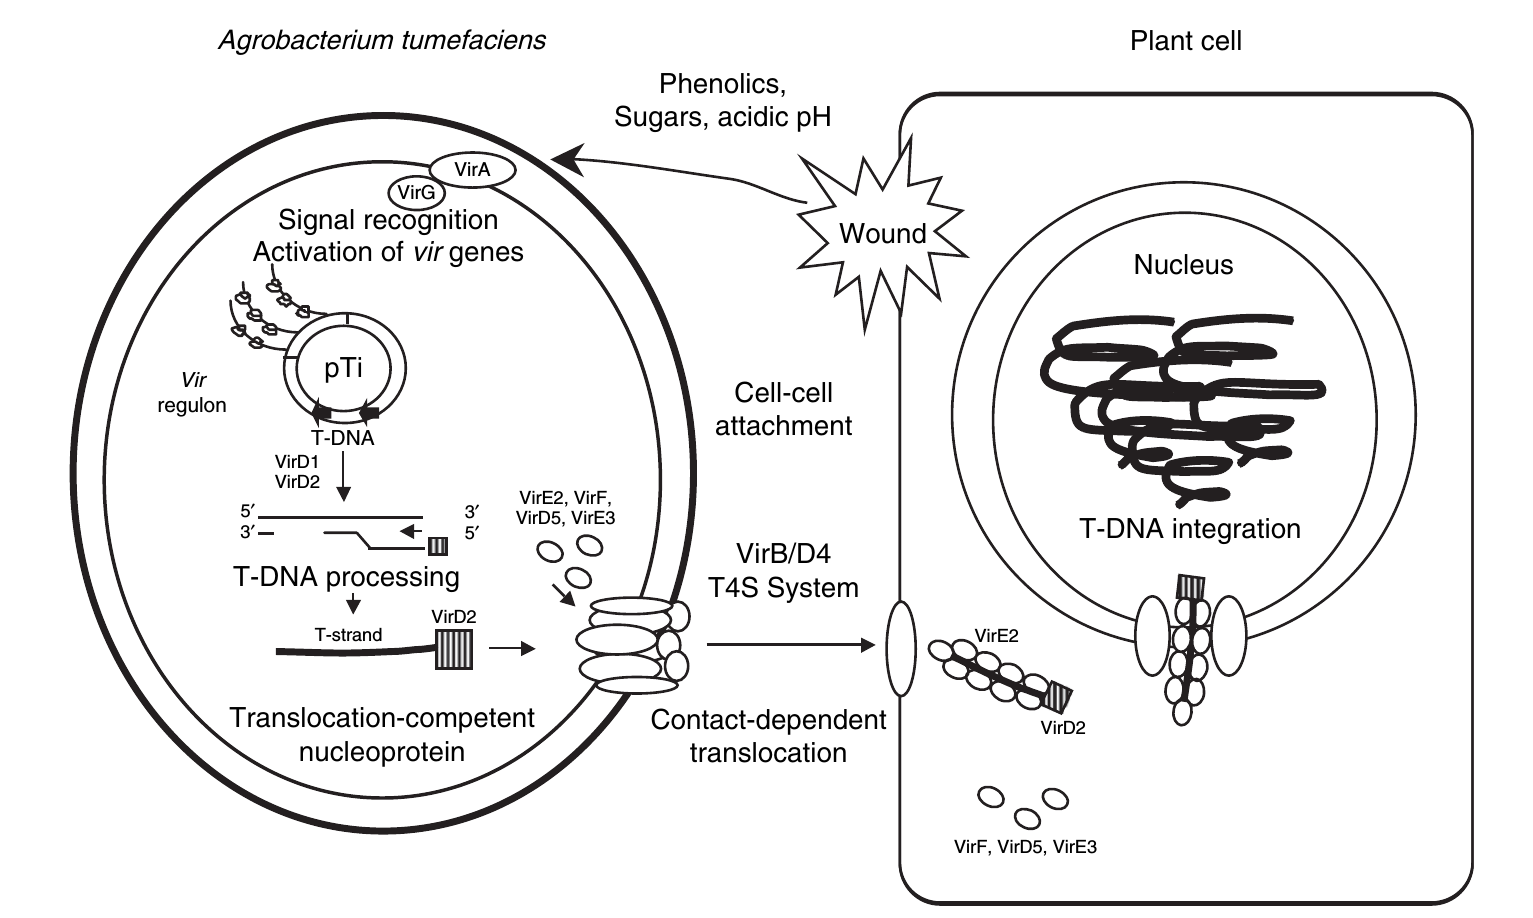
\includegraphics[width=0.66\linewidth]{../images/agrobacterium-transformation} 

}

\caption{Overview of agrobacterium tumefaciens infection process. Upon activation of the VirA/VirG two-component signal transduction system by signals released from wounded plant cells, a single-strand transferred DNA (T-DNA) is processed from the Ti plasmid and delivered as a nucleoprotein complex (T-complex) to plant nuclei. Expression of T-DNA genes in the plant result in the loss of cell growth control and tumor formation.}\label{fig:mechanism-of-infection}
\end{figure}
\end{frame}

\begin{frame}{}
\protect\hypertarget{section-5}{}
\begin{center}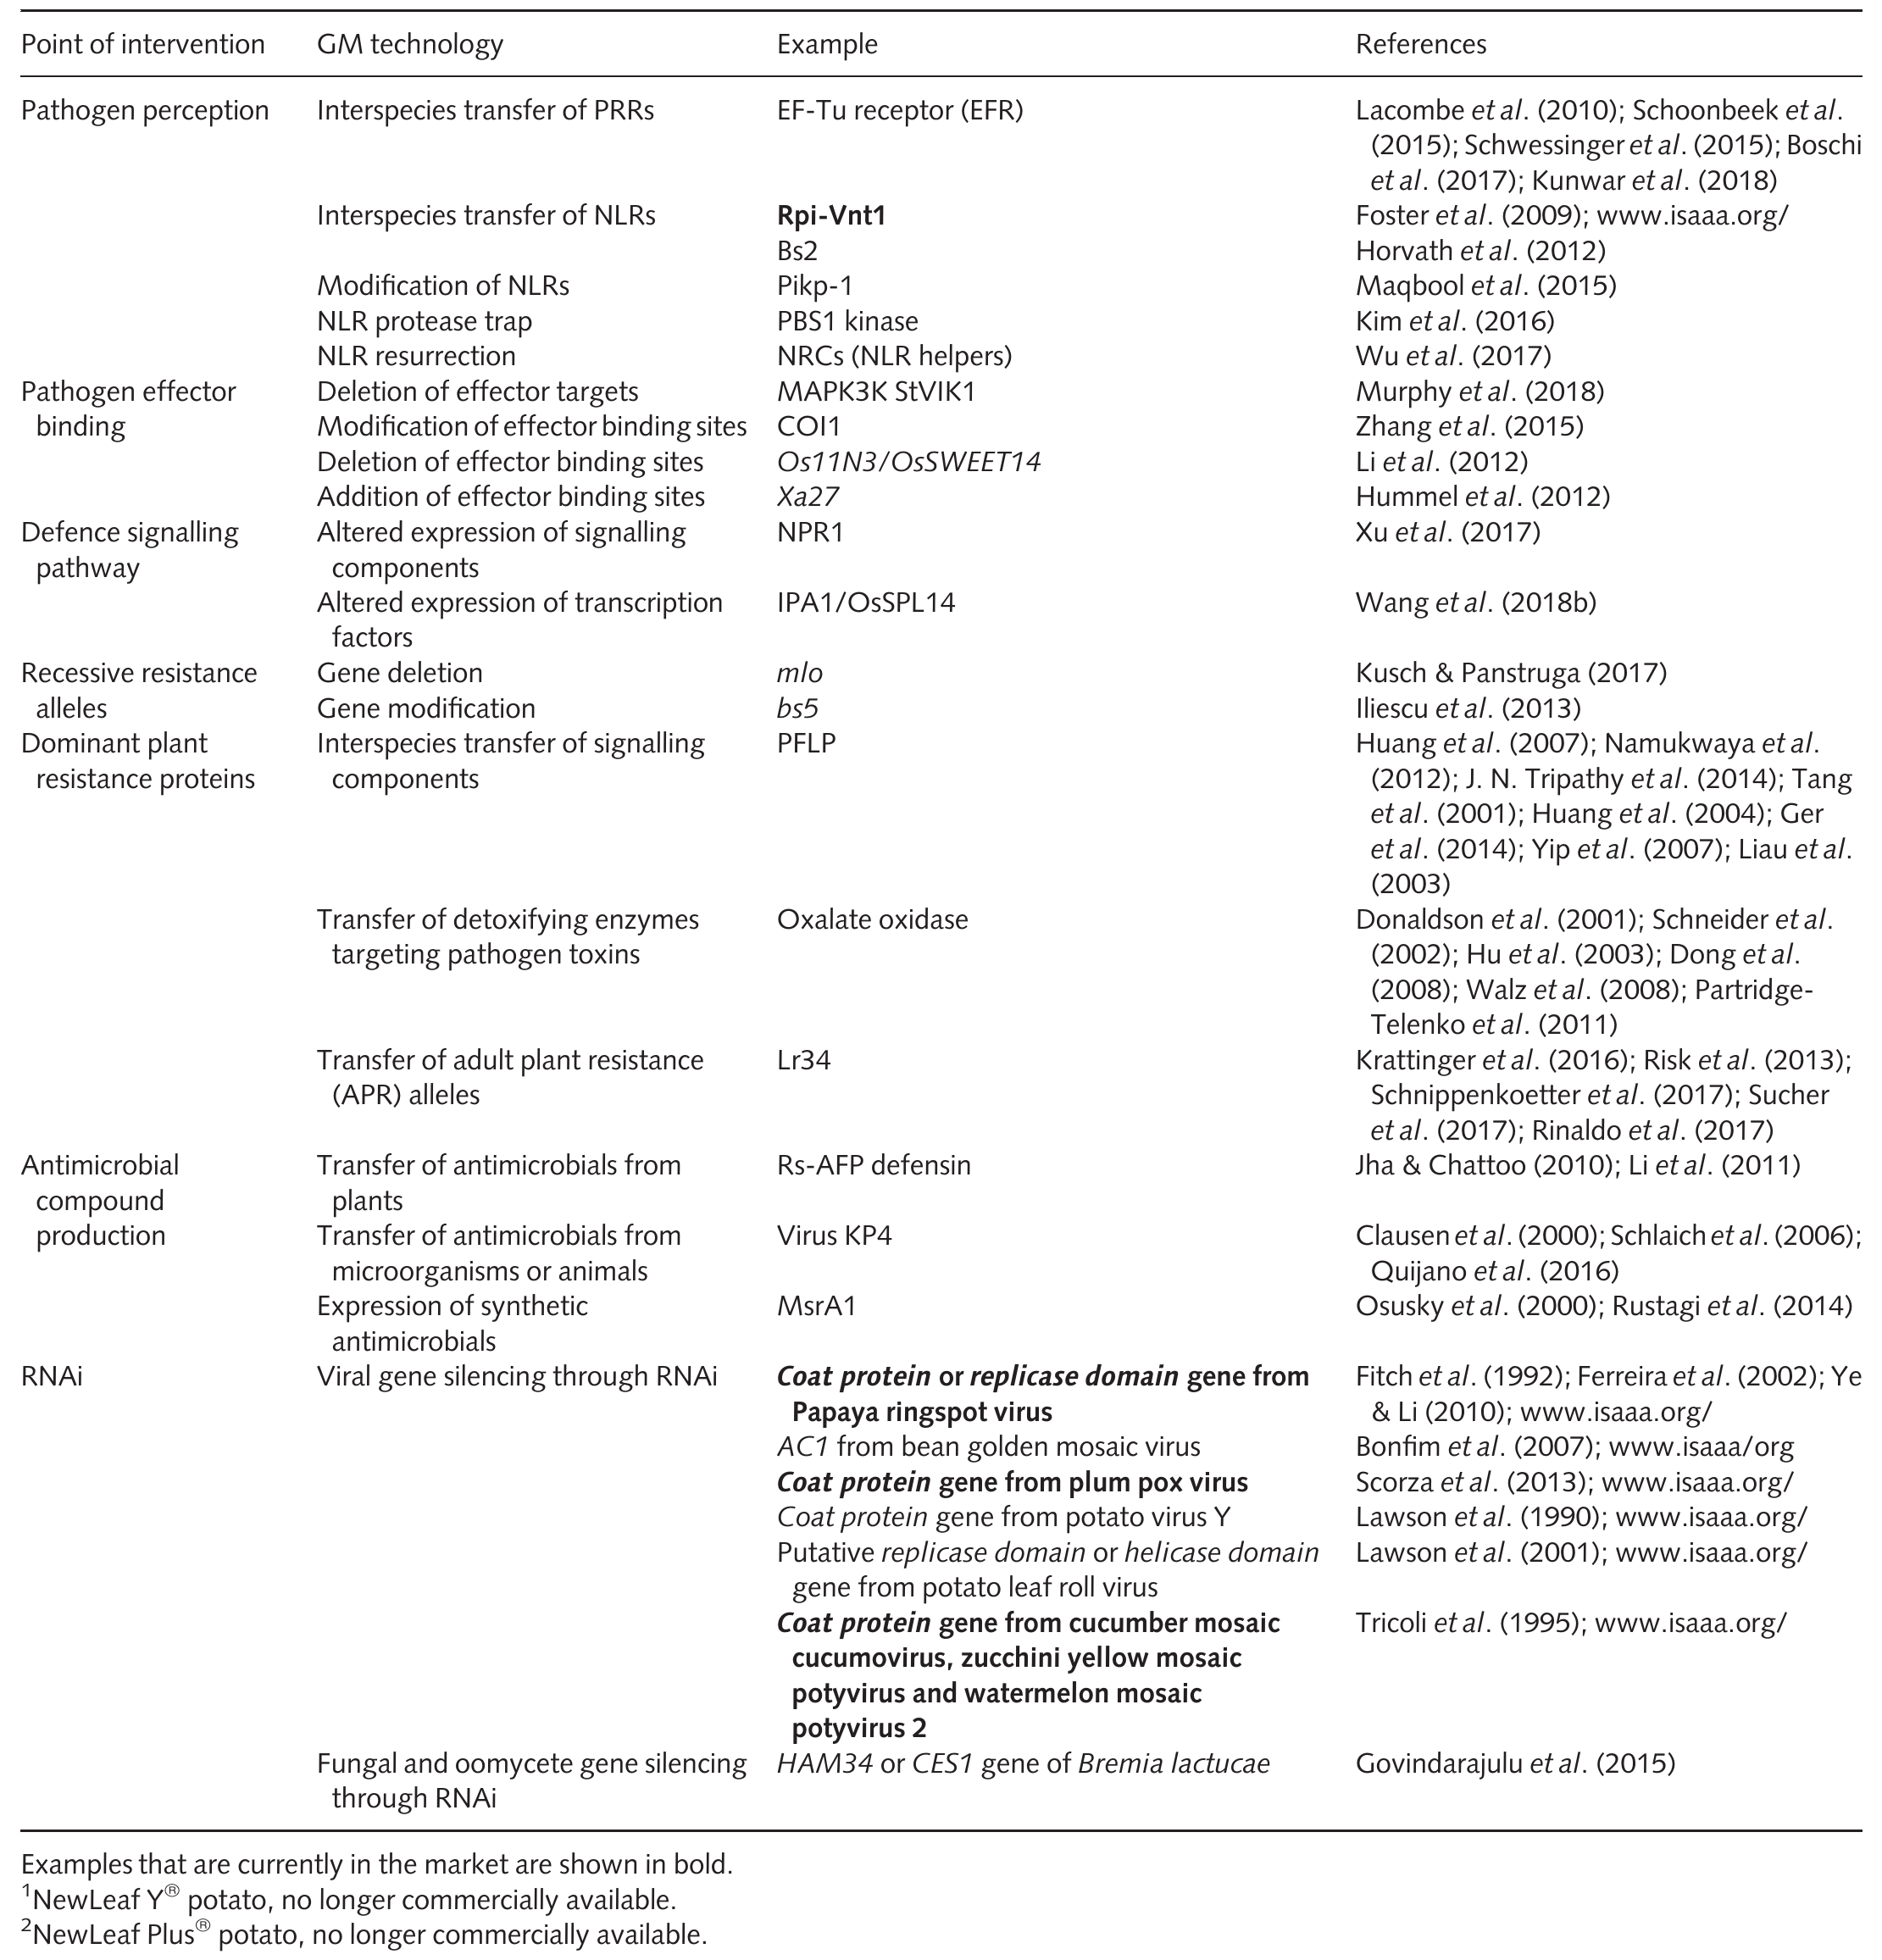
\includegraphics[width=0.4\linewidth]{../images/genetic_solution_pathogens} \end{center}

\tiny (Note: Refer to \citep{van2020genetic} for more on topic: Genetic
modification to improve disease resistance in crops.
\end{frame}

\hypertarget{gene-for-gene-hypothesis}{%
\section{Gene for gene hypothesis}\label{gene-for-gene-hypothesis}}

\begin{frame}{}
\protect\hypertarget{section-6}{}
\begin{itemize}
\tightlist
\item
  \citet{flor1956complementary} was the first to show there was a
  `gene-for-gene' relationship between the pathogen's avirulence (
  \emph{Avr}) genes and the resistance ( \emph{R}) genes of its host.
\item
  ``A resistance gene, \(R\) is only effective if the infecting pathogen
  carries the corresponding avirulence gene, \(A\)''.
\item
  Host resistance is conditioned by dominant allele, \(R\).
\item
  In the pathogen, virulence is conditioned by recessive allele, \(a\)
\item
  Resistance reaction occurs when complementary genes in both host and
  pathogen are dominant.
\item
  A host genotype that carries no dominant alleles at any of the loci is
  susceptible for all the races of pathogen (even if avirulent).
\item
  An \(A\) (avirulent) allele is dominant over \(a\) (virulent) allele
  and resistant allele \(R\) is dominant over susceptible allele \(r\).
\item
  Compatibility depends on the genotype of the host and the genotype of
  the pathogen.
\end{itemize}
\end{frame}

\begin{frame}{}
\protect\hypertarget{section-7}{}
\begin{columns}[T, onlytextwidth]
\column{0.4\textwidth}

\begin{table}

\caption{\label{tab:host-path-compatibility-mono}Host-pathogen compatibility reactions in monogenic resistance due to allelic variants of $R$ and $A$ genes. '-' symbol indicates incompatible reaction implying host immunity while '+' symbol denotes compatible interaction.}
\centering
\fontsize{6}{8}\selectfont
\begin{tabular}[t]{>{\raggedright\arraybackslash}p{8em}>{\raggedright\arraybackslash}p{6em}>{\raggedright\arraybackslash}p{6em}}
\toprule
\multicolumn{1}{c}{ } & \multicolumn{2}{c}{Pathogen genotype} \\
\cmidrule(l{3pt}r{3pt}){2-3}
Host genotype & A (avirulence) & a (non-avirulence)\\
\midrule
R (resistance) & - & +\\
r (susceptible) & + & +\\
\bottomrule
\end{tabular}
\end{table}

\column{0.6\textwidth}

\begin{table}

\caption{\label{tab:host-path-compatibility-tri}Host-pathogen compatibility reactions in trigenic resistance due to allelic variants of $R_1, R_2, R_3$ and $A_1, A_2, A_3$ genes. '-' symbol indicates incompatible reaction implying host immunity while '+' symbol denotes compatible interaction.}
\centering
\fontsize{6}{8}\selectfont
\begin{tabular}[t]{>{\raggedright\arraybackslash}p{7.5em}>{\raggedright\arraybackslash}p{2.2em}>{\raggedright\arraybackslash}p{2.2em}>{\raggedright\arraybackslash}p{2.2em}>{\raggedright\arraybackslash}p{2.2em}>{\raggedright\arraybackslash}p{2.2em}>{\raggedright\arraybackslash}p{2.2em}>{\raggedright\arraybackslash}p{2.2em}>{\raggedright\arraybackslash}p{2.2em}}
\toprule
\multicolumn{1}{c}{ } & \multicolumn{8}{c}{Pathogen genotype} \\
\cmidrule(l{3pt}r{3pt}){2-9}
Host haplotype & $A_1 A_2 A_3$ & $A_1 A_2 a_3$ & $A_1 a_2 A_3$ & $A_1 a_2 a_3$ & $a_1 A_2 A_3$ & $a_1 A_2 a_3$ & $a_1 a_2 A_3$ & $a_1 a_2 a_3$\\
\midrule
$R_1 R_2 R_3$ & - & - & - & - & - & - & - & +\\
$R_1 R_2 r_3$ & - & - & - & - & - & - & + & +\\
$R_1 r_2 R_3$ & - & - & - & - & - & + & - & +\\
$R_1 r_2 r_3$ & - & - & - & - & + & + & + & +\\
$r_1 R_2 R_3$ & - & - & - & + & - & - & - & +\\
\addlinespace
$r_1 R_2 r_3$ & - & - & + & + & - & - & + & +\\
$r_1 r_2 R_3$ & - & + & - & + & - & + & - & +\\
$r_1 r_2 r_3$ & + & + & + & + & + & + & + & +\\
\bottomrule
\end{tabular}
\end{table}

\end{columns}
\end{frame}

\begin{frame}{}
\protect\hypertarget{section-8}{}
\begin{table}
\centering\begingroup\fontsize{6}{8}\selectfont

\begin{tabular}{>{\raggedright\arraybackslash}p{5em}>{\raggedright\arraybackslash}p{6em}>{\raggedright\arraybackslash}p{5em}>{\raggedright\arraybackslash}p{7em}>{\raggedright\arraybackslash}p{7em}}
\toprule
Variety & Virus concentration & Yellowing & Yield with virus (kg) & Yield without virus (kg)\\
\midrule
A & 100 & 8 & 80 & 90\\
B & 60 & 5 & 100 & 110\\
C & 50 & 4 & 75 & 90\\
D & 70 & 6 & 50 & 100\\
\bottomrule
\end{tabular}
\endgroup{}
\end{table}

\begin{itemize}
\tightlist
\item
  Which variety is the most susceptible and why ?
\item
  Which variety is the most resistant and why ?
\item
  Which variety is the most tolerant and why ?
\item
  Which variety is the most sensitive and why ?
\end{itemize}
\end{frame}

\begin{frame}{}
\protect\hypertarget{section-9}{}
\begin{table}
\centering\begingroup\fontsize{7}{9}\selectfont

\begin{tabular}{>{\raggedright\arraybackslash}p{6em}>{\raggedright\arraybackslash}p{2.5em}>{\raggedright\arraybackslash}p{2.5em}>{\raggedright\arraybackslash}p{3.5em}>{\raggedright\arraybackslash}p{4.5em}}
\toprule
\multicolumn{1}{c}{ } & \multicolumn{2}{c}{Variety} & \multicolumn{2}{c}{Progeny ratio} \\
\cmidrule(l{3pt}r{3pt}){2-3} \cmidrule(l{3pt}r{3pt}){4-5}
Pathotype & A & B & F1 & F2\\
\midrule
P1 & R & S & All R & 3 R, 1 S\\
P2 & S & R & All R & 3 R, 1 S\\
P3 & R & R & All R & 15 R, 1 S\\
P1 + P2 & S & S & All R & 9 R, 7 S\\
\bottomrule
\end{tabular}
\endgroup{}
\end{table}
\end{frame}

\begin{frame}{}
\protect\hypertarget{section-10}{}
\begin{itemize}
\tightlist
\item
  Var \(A\): \(AAbb\)
\item
  Var \(B\): \(aaBB\)
\item
  \(F_1\): \(AaBb\)
\item
  \(P_1\): \(A_1 A_1 a_2 a_2\) (\(\because F_2\) ratio = \(3:1\))
\item
  \(P_2\): \(a_1 a_1 A_2 A_2\) (\(\because F_2\) ratio = \(3:1\))
\item
  \(P_3\): \(A_1 a_1 A_2 a_2\) (\(\because F_2\) ratio = \(15:1\),
  phenotype is due to duplicate gene action)
\item
  \(P_1 + P_2\): \(A_1 A_1 a_2 a_2 + a_1 a_1 A_2 A_2\) (\(\because F_2\)
  ratio = \(9:7\), phenotype is due to complementary gene action)
\end{itemize}
\end{frame}

\hypertarget{host-and-non-host-resistance}{%
\section{Host and non-host
resistance}\label{host-and-non-host-resistance}}

\begin{frame}{}
\protect\hypertarget{section-11}{}
\begin{columns}[T, onlytextwidth]
\column{0.5\textwidth}
\begin{itemize}
\small
\item Generally, the pathogen is specific to a certain infection of a host plant.
  \begin{itemize}
  \footnotesize
  \item \textit{F oxysporum} f. sp. \textit{lycopersici} is exclusive to tomato for tomato wilt
  \item \textit{Venturia inaequalis} only affects apple causing apple scab
  \item \textit{Puccinia graminis} f. sp. \textit{tritici} causing stem rust of wheat, attacks only wheat
  \end{itemize}
\item Development of disease in a host is conditioned by presence of one or more genes for pathogenicity, for specificity, and in pathogen the corresponding virulence gene
\end{itemize}

\column{0.5\textwidth}

\begin{figure}
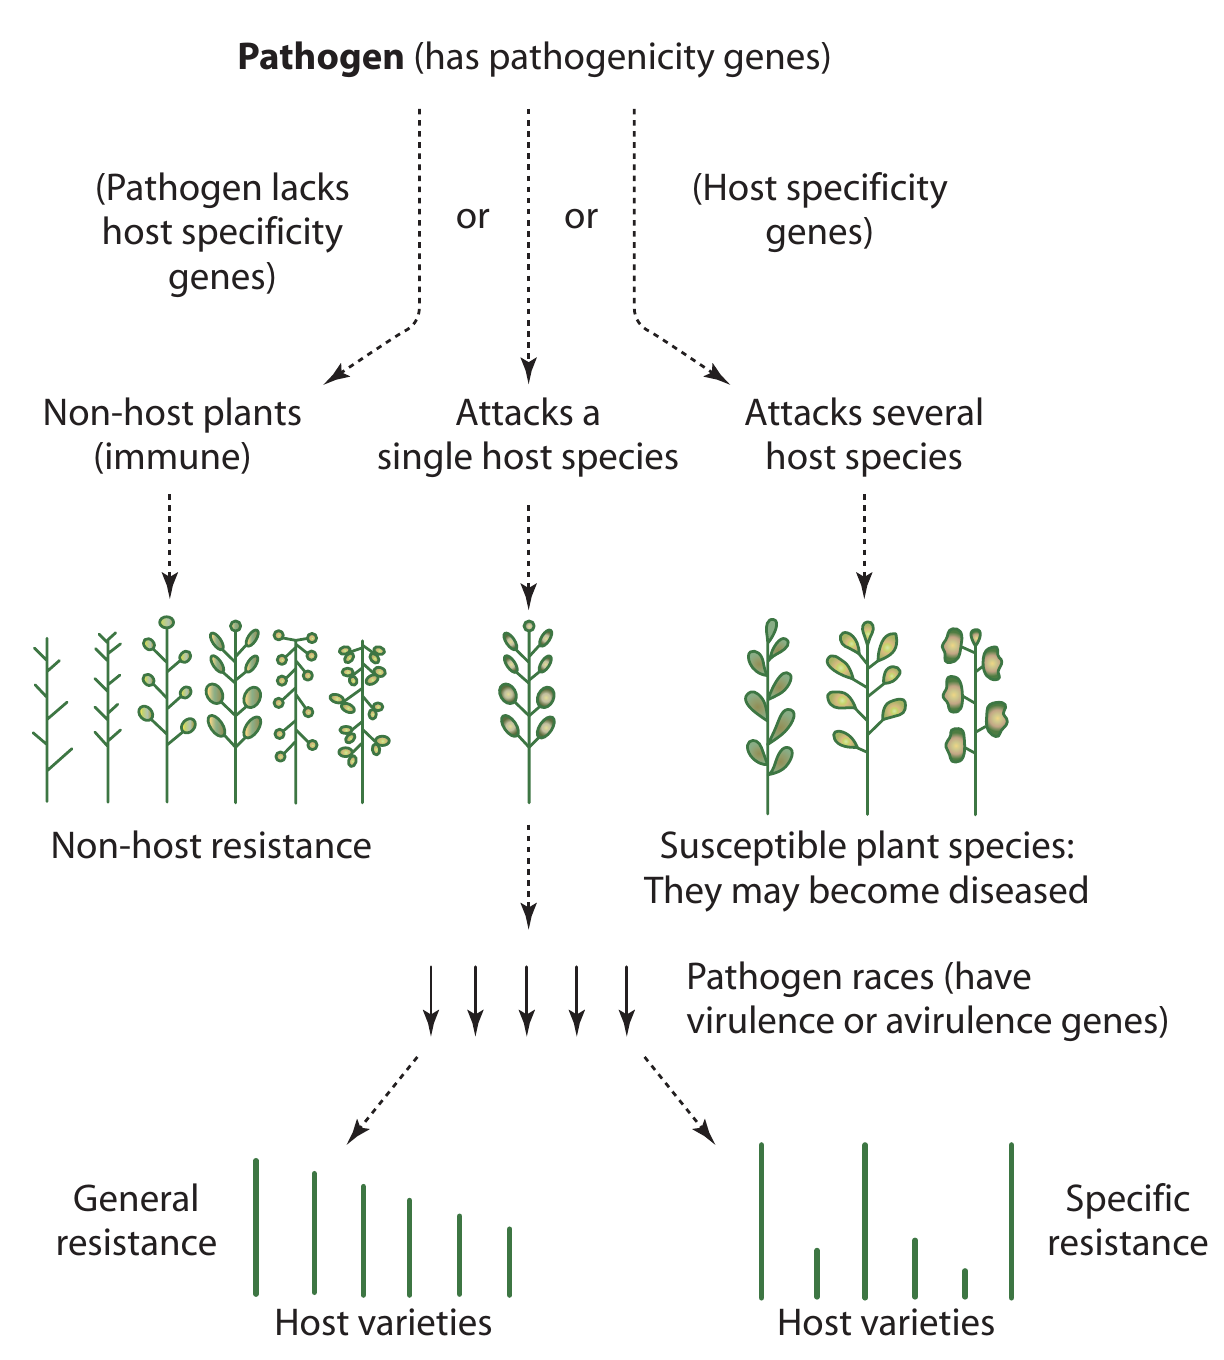
\includegraphics[width=0.7\linewidth]{../images/host_non_host} \caption{Gene interactions of a pathogen with its host and non-host plant}\label{fig:pathogen-host-non-host-interaction}
\end{figure}

\end{columns}
\end{frame}

\begin{frame}{}
\protect\hypertarget{section-12}{}
\begin{description}
\small
\item[Host range] List of plant species that can be exploited to be a natural enemy as source of nutrients.
\item[Generalists/polyphagous] Natural enemy with a wide host range.
\item[Specialits/oligophagous/monophagous] Natural enemy with a narrow host range or even single plant species.
\end{description}

\begin{itemize}
\tightlist
\item
  The complex of characters of a plant species that are responsible for
  making it a non-host to a certain potential natural enemy is non-host
  resistance.
\item
  No single individual plants of non-host species are susceptible to a
  natural enemy.
\end{itemize}
\end{frame}

\begin{frame}{}
\protect\hypertarget{section-13}{}
\small

\begin{itemize}
\tightlist
\item
  Non-host resistance (NHR) is largely modulated by PTI (discussed in
  Lecture: Introduction to Resistance Breeding)
\item
  NHR triggers multi-layered basal resistance mechanisms:

  \begin{itemize}
  \footnotesize
  \item peroxisome-based biosynthesis
  \item restriction of pathogen growth by nutrient limitation
  \item papilla formation
  \item callose and lignin deposition
  \end{itemize}
\item
  To contrast, genes involved in ETI pathways act on the basis of
  specific recognition, and develop hypersensitive response (HR)
  involving programmed cell death.
\item
  Many genes involved in NHR have multi-functional roles (including in)
  -- plant development
  (G-proteins\footnote[frame]{\scriptsize highly conserved heterotrimers proteins, mutation of which compromises NHR agaist fungal and bacterial pathogens}),
  stomatal regulation and plant metabolism.

  \begin{itemize}
  \footnotesize
  \item glycolate oxidase pathway
  \item proline dehydrogenase
  \end{itemize}
\item
  Both (above) enzymes modulate Reactive Oxygen Species (ROS) mediated
  signal transduction pathways in response to various environmental
  stresses! as well as providing NHR against bacterial pathogens.
\end{itemize}
\end{frame}

\begin{frame}{}
\protect\hypertarget{section-14}{}
\small

\begin{itemize}
\tightlist
\item
  NHR may be divided into 2 categories:

  \begin{itemize}
  \footnotesize
  \item Type I (does not show visible cell death symptoms)
  \item Type II (show localized hypersensitive response HR cell death, mediated through generation of ROS)
  \end{itemize}
\item
  NHR against pathogens of more closely related species can involve
  mechanisms more similar to host resistance

  \begin{itemize}
  \footnotesize
  \item maize resistance gene \textit{Rxo1} can recognize the rice bacterial streak pathogen
  \end{itemize}
\item
  Huanglongbing in citrus caused by vector-transmitted bacterial
  pathogen, \emph{Candidatus} spp. has been controlled through
  genetically modified alternative resistance gene from
  \emph{Arabidopsis thaliana}

  \begin{itemize}
  \scriptsize
  \item \textit{NPR1} gene transformed into sweet orange cultivars -- Hamlin and Valencia, and endogenous expression of \textit{AtNPR1} (targets signaling pathway for plant immunity) constitutively down-regulated\footnote[frame]{\scriptsize Refer to the article: The Arabidopsis AtNPR1 inversely modulates defense responses against fungal, bacterial, or viral pathogens while conferring hypersensitivity to abiotic stresses in transgenic rice, DOI: \url{https://doi.org/10.1094/mpmi-21-9-1215}}
  \end{itemize}
\end{itemize}
\end{frame}

\begin{frame}{}
\protect\hypertarget{section-15}{}
\small

\begin{itemize}
\tightlist
\item
  NHR resistance also sometimes provides broad spectrum resistance

  \begin{itemize}
  \footnotesize
  \item \textit{Rxo1} locus in maize confers resistance to all races of rice bacterial leaf streak pathogen \textit{Xanthomonas oryzae} pv. {oryzicola}.
  \item Tansgenic rice plants expressing \textit{Rxo1} showed strong resistance against \textit{X. oryzae} pv. {oryzicola}.
  \item This transgenic rice is resistant to another bacterial spot pathogen, \textit{Burkholderia andropogonis}.
  \end{itemize}
\item
  For breeding NHR mechanisms, steps are:

  \begin{itemize}
  \footnotesize
  \item screening of related species accessions (looking for susceptible individuals) among non-host species
  \item crossing and study of inheritance within non-host species to identify causal loci
  \item introgression of gene to host via hybridization with the non-host species, if possible
  \end{itemize}
\end{itemize}

\footnotesize

\begin{itemize}
\tightlist
\item
  Ideally, interfertile host as well as non-host species are hybridized
  and QTL mapping studies are conducted as in \textit{Bremia lactuca}.

  \begin{itemize}
  \scriptsize
  \item Lettuce downy mildew (causal: \textit{Bremia lactucae}) non-host \textit{Lactuca saligna} was crossed to host species \textit{L. sativa}, and backcross inbred lines were developed to stack alleles at four recessive NHR QTL\footnote[frame]{Refer to Genetic dissection of Lactuca saligna nonhost resistance to downy mildew at various lettuce developmental stages. DOI: \url{doi: 10.1111/j.1365-3059.2009.02066.x}}.
  \end{itemize}
\end{itemize}
\end{frame}

\hypertarget{defense-mechanisms-against-insects}{%
\section{Defense mechanisms against
insects}\label{defense-mechanisms-against-insects}}

\hypertarget{bibliography}{%
\section{Bibliography}\label{bibliography}}

\begin{frame}{References}
\protect\hypertarget{references}{}
\end{frame}

          \begin{frame}[allowframebreaks]{}
    \bibliographytrue
    \bibliography{./../bibliographies.bib}
    \end{frame}
  


\end{document}
